\documentclass[sigplan,screen]{acmart}

\usepackage[ruled]{algorithm2e}
\usepackage{graphicx}
\usepackage{hyperref}

\graphicspath{ {./images/} }

\renewcommand{\algorithmcfname}{ALGORITHM}
%% Remove Permissions and ACM Reference Notes
\renewcommand\footnotetextcopyrightpermission[1]{}
\settopmatter{printacmref=false}
%%
%% \BibTeX command to typeset BibTeX logo in the docs
\AtBeginDocument{%
  \providecommand\BibTeX{{%
    \normalfont B\kern-0.5em{\scshape i\kern-0.25em b}\kern-0.8em\TeX}}}

\begin{document}

\title{Árvores Minimax}
\subtitle{DIM0806 - Estruturas de Dados e Algoritmos}

\author{Tiago Vinícius Remígio da Costa}
\email{vinicius.remigio@gmail.com}
\affiliation{
  \institution{DIMAp - Universidade Federal do Rio Grande do Norte}
  \city{Natal}
  \state{RN}
  \country{Brasil}
}

\begin{abstract}
  Árvores minimax têm sido usadas no estudo de jogos de soma zero.
  Neste artigo veremos algumas implicações desta estrutura de dados, 
  assim como pseudo-código do algoritmo para encontrar o melhor estado ,complexidade, trade-offs e exemplos de utilização. 

  Para tornar o conceito mais didático, será mostrada uma implementação usando o Jogo da Velha {\itshape(Tic Tac Toe)}, onde dois jogadores se enfrentam.

  Também será vista uma implementação da poda alfa-beta, para reduzir o espaço de buscas.
\end{abstract}

\keywords{algoritmos, estruturas de dados, árvores, teoria dos jogos, minimax, soma zero}

\maketitle
\pagestyle{plain}

\section{Introdução}

Jogos têm servido de inspiração para o estudo da inteligência artificial desde os anos 50 a partir dos primeiros programas de jogos de xadrez escritos por Claude Shannon e Alan Turing. 
Estados de um jogo, como Chess e Go, são facilmente representados e os agentes inteligentes possuem um conjunto finito de ações \cite{russel2010}. 
O fato desses agentes serem adversários introduz um componente de incerteza, já que esses oponentes não sabem qual a ação a ser tomada pelo seu adversário.

O Minimax escolhe uma jogada ótima para um jogador, assumindo que seu adversário também realiza jogadas de maneira ótima \cite{Jain17}.
Obter algoritmos que calculem uma estratégia capaz de recomendar uma ação para qualquer estado. 
O algoritmo minimax é usado em tomada de decisões, encontrando uma jogada ótima para um jogador, assumindo que seu oponente também joga de forma ótima.

Além disso, a pode permite ignorar ramos da árvore que não fazem diferença no resultado final, e funções heurísticas permitem a aproximação da utilidade de um estado sem a necessidade de realizar uma busca exploratória.

As outras seções deste artigo são o conceito de soma zero, uma análise sobre o algoritmo minimax, incluindo pseudocódigo, Complexidade e um exemplo aplicado ao Jogo da Velha (Tic Tac Toe). 
Por fim, veremos alguns trade-offs, o que nos leva a poda alfa-beta. Também serão listadas algumas aplicações e as conclusões do trabalho.

\subsection{Soma Zero}
Em um jogo determinístico de soma zero, o placar final de um jogo em que dois jogadores são adversários.
Com o pressuposto da soma zero, os jogadores possuem utilidades opostas. Isso permite que a função heurística de utilidade seja a mesma.
Para cada jogador pode ser vitória {\itshape(1 ponto)}, empate {\itshape(0 pontos)} ou derrota {\itshape(-1 ponto)}, onde a soma das utilidades para ambos é sempre zero.

Os métodos de busca são sempre adversários, puramente competitivos, onde cada jogador está tentando ganhar e também provocando a derrota do oponente. 
O jogador que tenta ganhar é chamado de {\itshape maximizador (MAX)}, tentando maximizar seu score, enquanto o oponente é chamado de {\itshape minimizador (MIN)}, tentando minimizar o score do maximizador \cite{Aradhya01}.

Cada jogador possui a informação completa, ou seja, tem a visão das jogadas realizadas pelo adversário. Os jogos são realizados em turno, ou seja, cada jogado possui a sua vez de jogar.

Por ser uma técnica importante na IA para estudo de jogos adversários, muitos trabalhos com variações do minimax têm sido apresentados na literatura \cite{Diderich93} no decorrer dos anos.

\section{Minimax}
Em uma busca minimax, a árvore representa o espaço de estados, onde os jogadores se alternam nos movimentos. O valor minimax é computado para cada nó, buscando a melhor utilidade contra um agente adversário ótimo, que jogue de forma racional.

A idéia do Minimax é determinar uma estratégia ótima para o jogador MAX e então decidir o melhor primeiro movimento.

Todos os estados possuem um valor associado, onde o maximizador realiza uma jogada para aumentá-lo e o minimizador realiza uma jogada para diminuí-lo. 
O valor é calculado através de uma heurística, chamada de função de utilidade.

Para definir Minimax, necessitaremos de alguns conceitos:

\begin{itemize}
  \item \textbf{Estados inicial}: posição dos movimentos no tabuleiro;
  \item \textbf{Operadores}: movimentos válidos que um jogador pode fazer;
  \item \textbf{Estados de parada (terminais)}: Estados que determinam o fim do jogo;
  \item \textbf{Função de utilidade}: Retorna um valor númerico para o jogo, representando vitória, derrota ou empate.
\end{itemize}

\subsection{Algoritmo Minimax}

A figura \ref{ttt_parctree} mostra uma árvore parcial das jogadas para o Jogo da Velha (Tic-Tac-Toe), 
que será utilizado para exemplificar o funcionamento do Minimax.

\begin{figure}[h]
  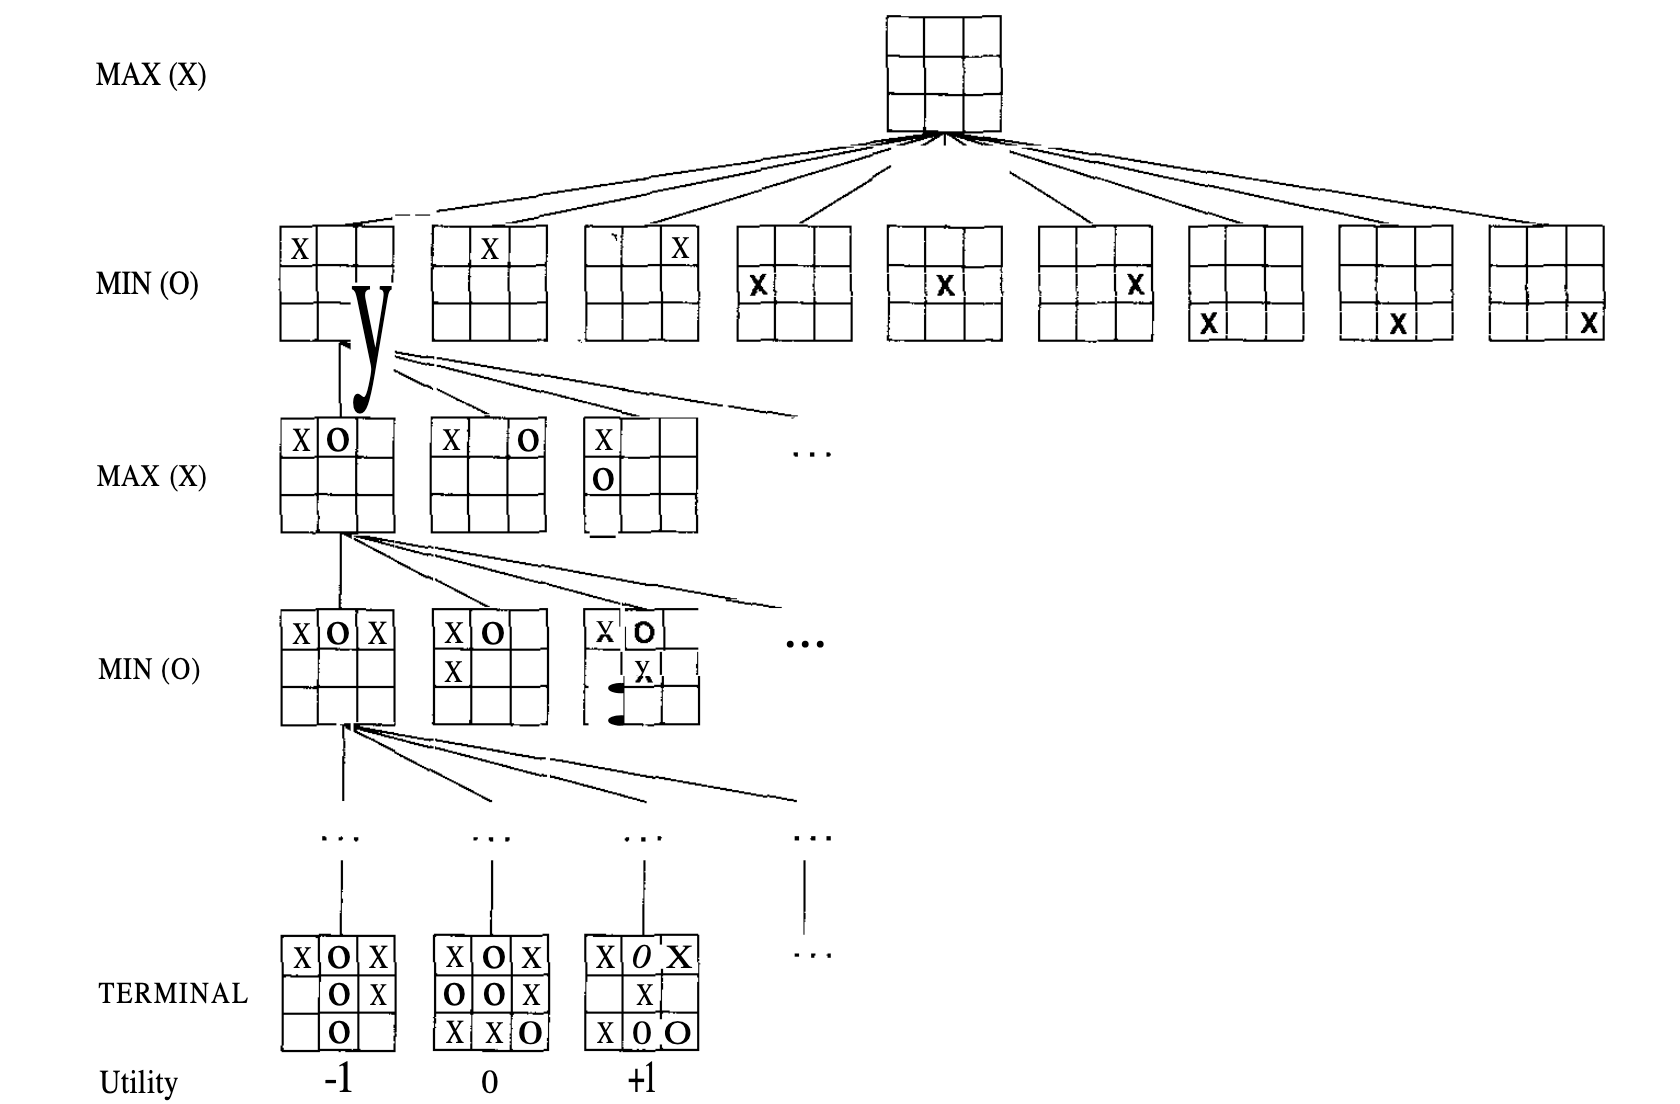
\includegraphics[width=8cm]{tictactoe_tree.png}
  \caption{Árvore parcial para o jogo da velha}
  \label{ttt_parctree}
\end{figure}

Aplicando os conceitos de Minimax que vimos anteriormente, temos que:

\begin{itemize}
  \item \textbf{Estados inicial}: tabuleiro vazio, onde o jogador MAX fará a primeira jogada;
  \item \textbf{Operadores}: O jogador MAX pode marcar um {\itshape X} em uma posição vazia, enquanto o jogador MIN pode marcar o {\itshape O};
  \item \textbf{Estados de parada (terminais)}: Estados que determinam o fim do jogo, que pode ser a vitória de MAX por sequência de {\itshape XXX} em linha, coluna ou diagonal. 
  Também pode ser a derrota de MAX e finalmente um empate;
  \item \textbf{Função de utilidade}: Retorna {\itshape +1} para a vitória de MAX, {\itshape -1} para a derrota de MAX ou {\itshape 0} para empate.
\end{itemize}

Portanto, o algoritmo Minimax pode ser resumido nos seguintes passos:

\begin{itemize}
  \item Gerar a árvore, a partir da raíz, que representa o estado inicial até os estados terminais;
  \item Aplicar a função de utilidade em cada estado terminal para computar o valor;
  \item Usar a função de utilidade para determinar a utilidade dos nós um nível acima na árvore de busca;
  \item Calcular o valor dos nós filhos até a raíz, uma camada por vez;
  \item MAX escolhe o movimento que leva ao maior valor.
\end{itemize}

\subsection{Pseudocódigo}
O pseudocódigo do algoritmo Minimax a seguir descreve o básico funcionamento do algoritmo. 
\footnote{A implementação do algoritmo pode ser encontrada em \href{https://bit.ly/3jc3wH0}{https://bit.ly/3jc3wH0}}
As funções {\itshape minValue} e {\itshape maxValue} possuem o mesmo funcionamento, apenas invertendo a lógica.


\begin{algorithm}
\DontPrintSemicolon
  \caption{Algoritmo Minimax}
  \label{alg:generator}
  \SetKwProg{minimax}{Function \emph{minimax}}{}{end}
  \minimax{Object state, Player player}{
    \If{ state is final}{
        \Return{state}\;
    }
    \If{player is MAX}{
      init v = -inf\;
      \ForEach{successor in s}{
        v = max(v, minimax(state=successor, player=MIN))\;
      }
    \KwRet{v}\;
    }
    \ElseIf{player is MIN}{
      init v = +inf\;
      \ForEach{successor in s}{
        v = min(v, minimax(state=successor, player=MAX))\;
      }
    \KwRet{v}\;
    }
  }
\end{algorithm}

A árvore minimax da figura \ref{tictactoe} foi gerada pela implementação do algoritmo descrito. 
Para simplificar a visualização, o estado inicial considerado {\itshape(Depth 0)} já possui algumas jogadas.

\begin{figure}[h]
  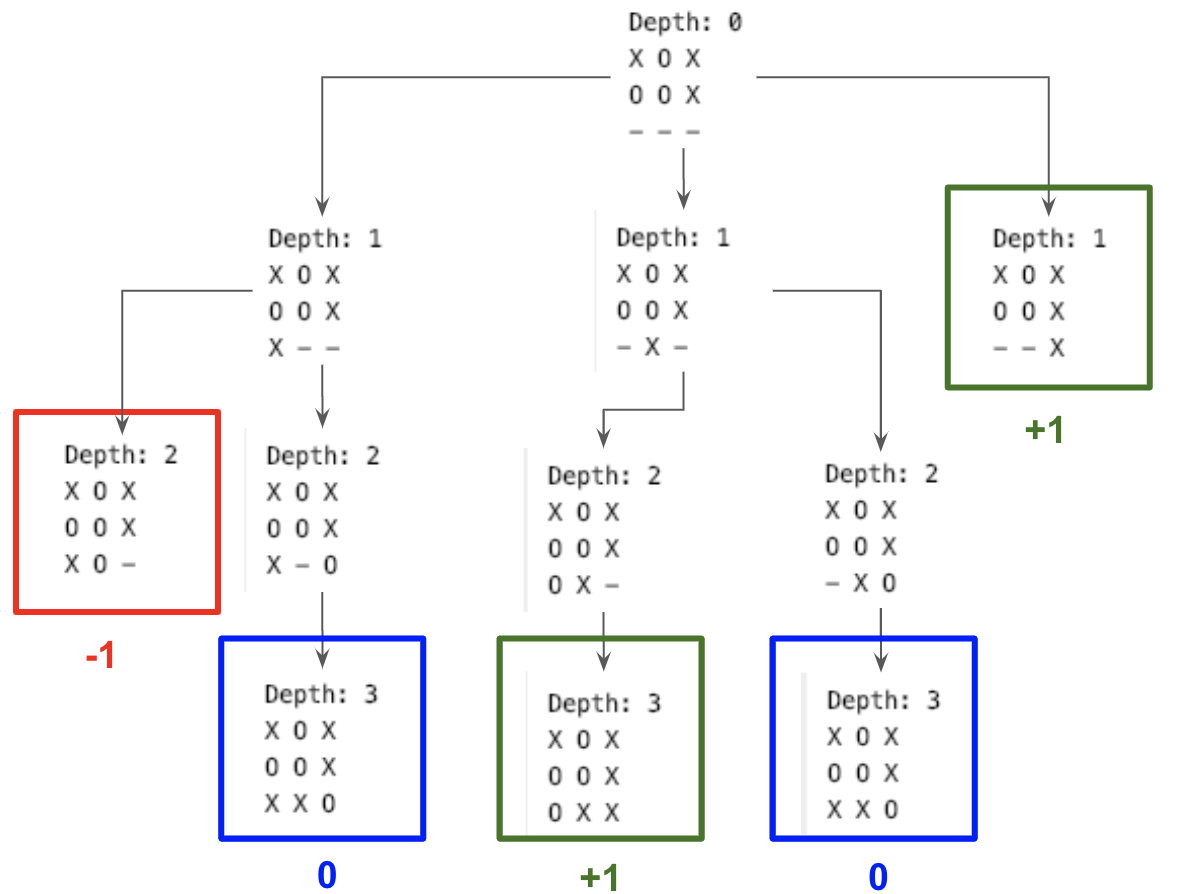
\includegraphics[width=8cm]{minimax_tree_1.png}
  \caption{Árvore MiniMax para um jogo da Velha, dado um estado inicial}
  \label{tictactoe}
\end{figure}

\subsection{Complexidade}

Possui a mesma complexidade que a busca em profundidade {\itshape (depth-first search)}, tornando inviável quando a árvore é profunda.
Considerando que m é a profundidade máxima da árvore e b é a quantidade de movimentos válidos em cada ponto, temos que:
\begin{itemize}
  \item Complexide de tempo: $O(b^m)$
  \item Complexidade de espaço: $O(bm)$
\end{itemize}

Em termos práticos, esta complexidade de tempo é impraticável.
Para minimizar um pouco deste problema, técnicas de poda, como a alfa-beta, são necessárias para trabalhar como representação Minimax, como será mostrado na próxima seção.


\section{Trade-offs}

Existe um trade-off entre a acurácia da função de avaliação e o custo do tempo de execução.  A maioria dos jogos usam uma função de avaliação linear.
No caso do Jogo da Velha, a função de avaliação verifica as linhas, colunas e diagonais procurando se MAX venceu, se MIN venceu, ou se as jogadas se esgotaram, caracterizando o empate.

Em problemas reais, é impossível computacionalmente buscar até as folhas, dada a profundidade da árvore e quantidade de estados gerados.
Uma solução possível é trabalhar com busca em profundidade limitada, criando por uma função de avaliação para posições que não são folhas.
Não há garantia que o resultado será ótimo, por isso aumentar a profundidade faz bastante diferença.

Se a profundidade for maior, a complexidade da função de avaliação pode ser menor. Mas se a poda for mais rasa, a função de avaliação precisaria ser mais complexa. 
Acarretando maior capacidade de computação. 
O ideal é chegar uma ponderação na qual consiga-se descer para uma maior profundidade e que a função não seja muito complexa de calcular.

\subsection{Poda Alfa-Beta}
É uma técnica de otimização para o algoritmo Minimax para reduzir o tempo de computação, por meio de podar ramos (branches) da árvore por previamente detectar movimentos melhores disponíveis \cite{Aradhya04}.
Assumindo que uma função de avaliação foi implementada junto a uma busca minimax, mesmo assim, o espaço de jogadas a frente ficará bastante limitado, se há a necessidade de percorrer toda a árvore.
Daí vem o conceito da poda: uma forma de tomar uma decisão minimax correta sem precisar percorrer toda a árvore, buscando não computar ramificações que possivelmente não interferem na decisão minimax.

Ao aplicar a poda alfa-beta, a complexidade do algoritmo tende a cair de $O(b^m)$ para $O(b^{m/2})$ para encontrar o melhor movimento.


\section{Aplicações}
Por ser bastante didático, o Minimax é muito utilizado em modelagem de problemas de jogos adversários, como jogo da velha, go, xadrez, damas entre outros jogos e situações onde dois jogadores/agentes inteligentes são adversários.
Esses jogos possuem em comum a possibilidade de ver claramente cada jogada dos jogadores. Além disso, toda informação do tabuleiro está sempre exposta.

\section{Conclusões}
O algoritmo Minimax utiliza árvores como estrutura de dados e busca representar dois agentes que buscam vencer, provocando a derrota do outro, em um jogo de soma zero. 
Este conceito têm sido bastante estudado na Economia, através da Teoria dos Jogos. 
Como a maioria das decisões ótimas de jogos são intratáveis, algoritmos precisam lidar com premissas e aproximações.

Na prática, a geração dos estados é extremamente custosa computacionalmente. Técnicas como a poda alfa-beta podem ajudar, eliminando ramos da árvore que não impactam no resultado final.

\bibliographystyle{ACM-Reference-Format}
\bibliography{sample-base}

\end{document}
\endinput
